%% source: 2023-sp-midterm_01
\begin{prob}
    Suppose the numbers
        \python{41},
        \python{32},
        and
        \python{33}
    are inserted (in that order) into the below binary search tree. Draw where
    the new nodes will appear.

    \vspace{1em}
    \begin{center}
    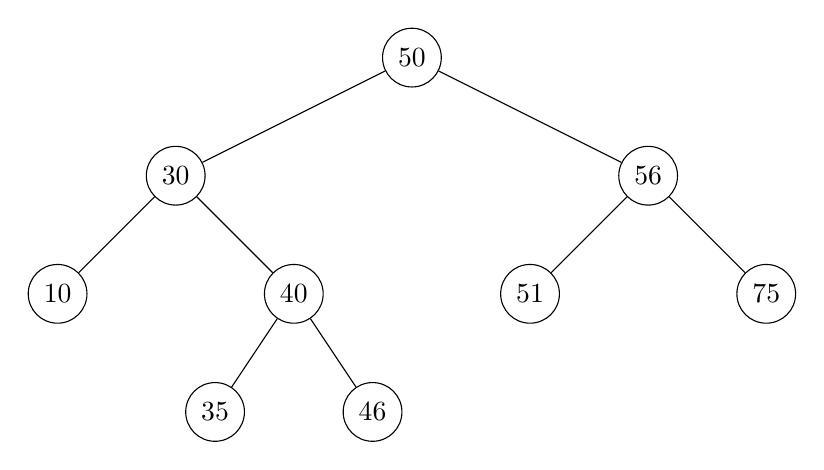
\begin{tikzpicture}[
            every node/.style={circle, draw},
            level 1/.style={sibling distance=60mm},
            level 2/.style={sibling distance=30mm},
            level 3/.style={sibling distance=20mm}
        ]
        \node (z){ 50 }
            child { node (a) { 30 }
                child { node (c) { 10 } }
                child { node (d) { 40 }
                    child { node (f) { 35 } }
                    child { node (f) { 46 } }
                }
            }
            child { node (b) { 56 }
                child { node (e) { 51 } }
                child { node (e) { 75 } }
            };
    \end{tikzpicture}
    \end{center}

\end{prob}
